\chapter{Anlyse et recommandations}
\label{chap:4}
\sloppy

\section{Analyse des cas de succès et d'échec}

Dans l'ensemble, il a été observé qu'une classe, à savoir AFV, a bien fonctionné dans nos deux expériences.
La raison en est que cette classe avait plus de données d'entraînement que les autres classes.
Les détails de notre ensemble de données proposé sont donnés dans le tableau \ref{tab:label_data}.
Au cours de l'analyse, nous avons observé que le système avait de bonnes performances sur les cas de test sur les images avec des véhicules visibles, mais il y avait des difficultés dans certains cas pour lesquels nous avions un petit jeu de données d'entraînement.
Il fonctionne bien sur les véhicules militaires dans les données non vues par rapport aux autres véhicules militaires car le rapport entre ses données d'entraînement est plus élevé.

Le modèle commence à mal fonctionner sur des données. Cela est dû au fait qu'il y a moins de données d'entraînement par rapport à l'autre classe.

\begin{table}[h]
    \centering
    \begin{tabular}{|l|l|l|p{2.8cm}|p{2cm}|p{2cm}|p{2cm}|}
        \hline
        \textbf{Label} & \textbf{Quantité} & \textbf{Pourcentage} & \textbf{Modèles} & \textbf{Précision moyenne} & \textbf{Recall Moyen} & \textbf{F1-Score Moyen} \\ \hline
        AFV            & 6694              & 82.5\%               & YoloV8 (m et l)  & 0.71                       & 0.676                 & 0.69                    \\ \hline
        APC            & 1212              & 15.0\%               & YoloV8 (m et l)  & 0.58                       & 0.544                 & 0.557                   \\ \hline
        LAV            & 374               & 4.6\%                & YoloV8 (m et l)  & 0.52                       & 0.464                 & 0.49                    \\ \hline
        MEV            & 123               & 1.5\%                & YoloV8 (m et l)  & 0.29                       & 0.530                 & 0.374                   \\ \hline
    \end{tabular}
    \caption{Tableau des moyennes des résultats}
    \label{tab:label_data}
\end{table}


\section{Limites et perspectives}
\subsection{Modèle de détection d'objets}
Ici, le modèle YoloVx, grâce à plusieurs contributions, a connu un gain de performance considérable durant ces dernières années.
Nous avons des scores de précision d'environ 80\% malgré la faible quantité de données utilisée pour l'entraînement du modèle.
Néanmoins, les paramètres (hyperparamètres) de ces modèles deviennent plus complexe à comprendre et à personnaliser et à améliorer afin d'obtenir des résultats optimales adapter à nos besoins.
A ce jour, par rapport à nos contraintes en détection de véhicules militaires, YoloVx c'est le modèle de détection me plus performant.
Nous allons continuer à ajuster les paramètres pour obtenir un modèles beaucoup plus performant.

\subsection{Augmentation des données}
\subsubsection{Transformation des images}
Dans cette étapes, nous appliquons trois transformations (scale, XYMasking, et Météo).
Grâce à cette méthode, en l'appliquant sur toutes les images du jeu de données, nous avons presque doublé leur nombre ainsi que leur annotation pour l'entraînement de notre modèles.

Nous avons fait un contrôle de qualité des images,nous avons constaté qu'il ya des images impossibles à lire.
Le tri de ces images n'est pas envisageable au vue de la quantité (3335) d'images du jeu de données sur le quel les transformations ont été appliquées.


\begin{figure}[H]
    \centering
    \begin{subfigure}[b]{0.45\textwidth}
        \centering
        
\includegraphics[height=5cm]{./images/augmented-1.jpg}
    \end{subfigure}
    \hfill
    \begin{subfigure}[b]{0.45\textwidth}
        \centering
        
\includegraphics[height=5cm]{./images/augmented-2.jpg}
    \end{subfigure}
    \vskip\baselineskip
    \begin{subfigure}[b]{0.45\textwidth}
        \centering
        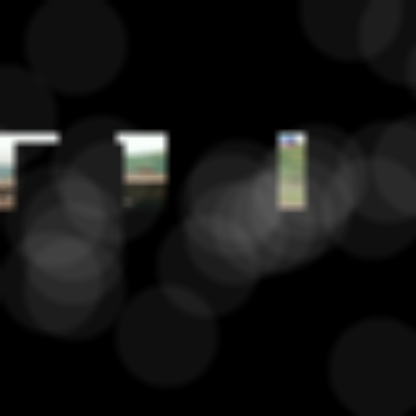
\includegraphics[height=5cm]{./images/augmented-3.jpg}
    \end{subfigure}
    \hfill
    \begin{subfigure}[b]{0.45\textwidth}
        \centering
        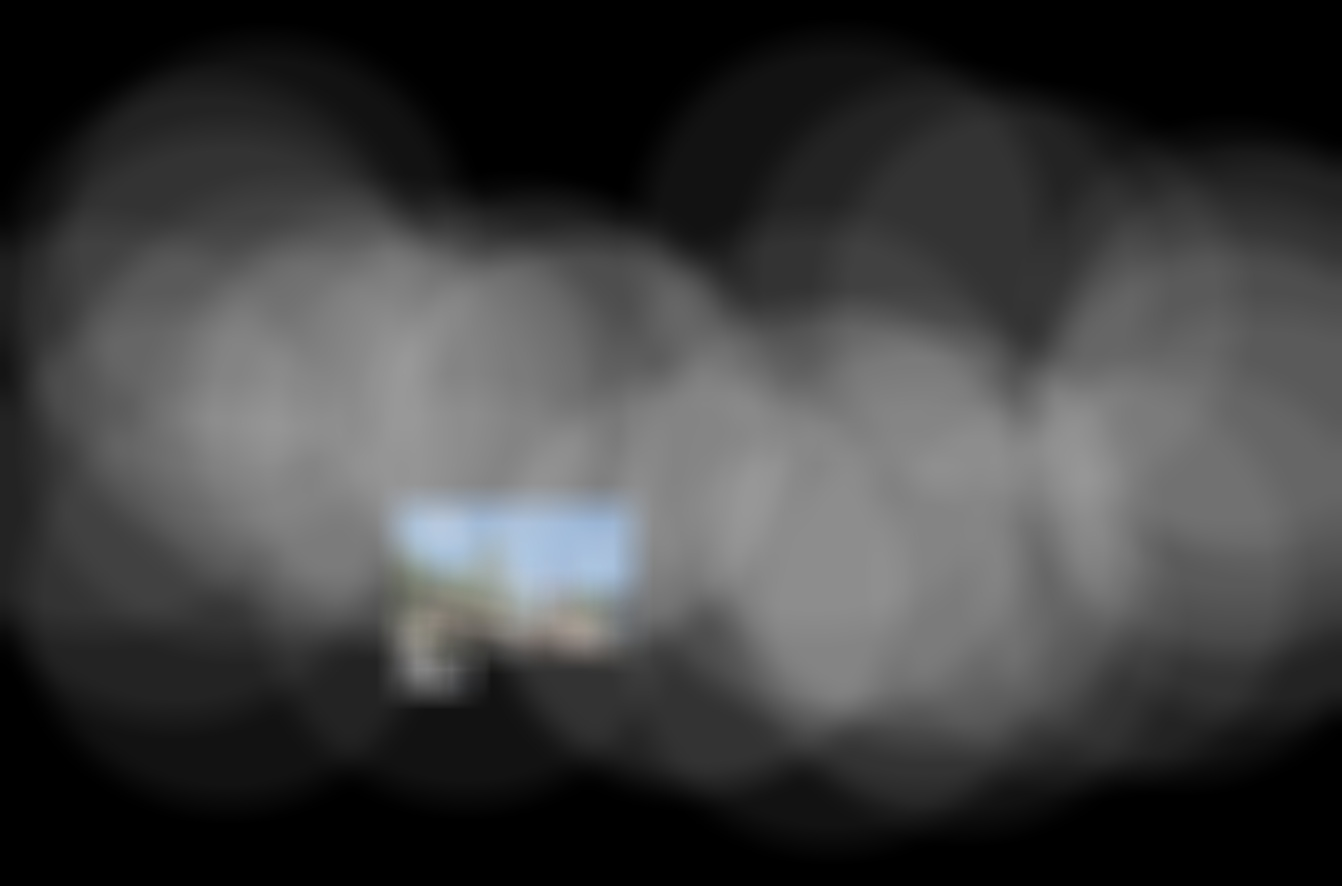
\includegraphics[height=5cm]{./images/augmented-4.JPEG}
    \end{subfigure}
    \caption{Exemples d'images transformées de véhicules militaires inexploitables}
\end{figure}


\subsubsection{Génération d'images}

La génération d'image nous permet d'augmenter le nombre de véhicules de notre jeu de données.
Comme inconvénients, sous pouvons citer :

\begin{itemize}
    \item Elle ne peut générer qu'un seul type de véhicule.
    \item Beaucoup d'images ne sont pas réalistes par conséquent inexploitables.
    \item Les images ne sont pas annotées et nécessite une annotation manuelle.
    \item Aucun moyen d'évaluer objectivement la qualité du rendu. Tout est subjectif, donc fastidieux.
\end{itemize}

\begin{quote}
    % \textit{Si vous recherchez un certain résultat dans votre art, déterminer si un modèle est sur ou sous-entraîné sera toujours subjectif, car l'art est subjectif.}\\
    \textit{If you are going for a certain result in your art, then determining if a model is over or under trained is always going to be subjective, because art is subjective.\cite{reddit_proverbe}}
\end{quote}


\begin{figure}[H]
    \centering
    \begin{subfigure}[b]{0.45\textwidth}
        \centering
        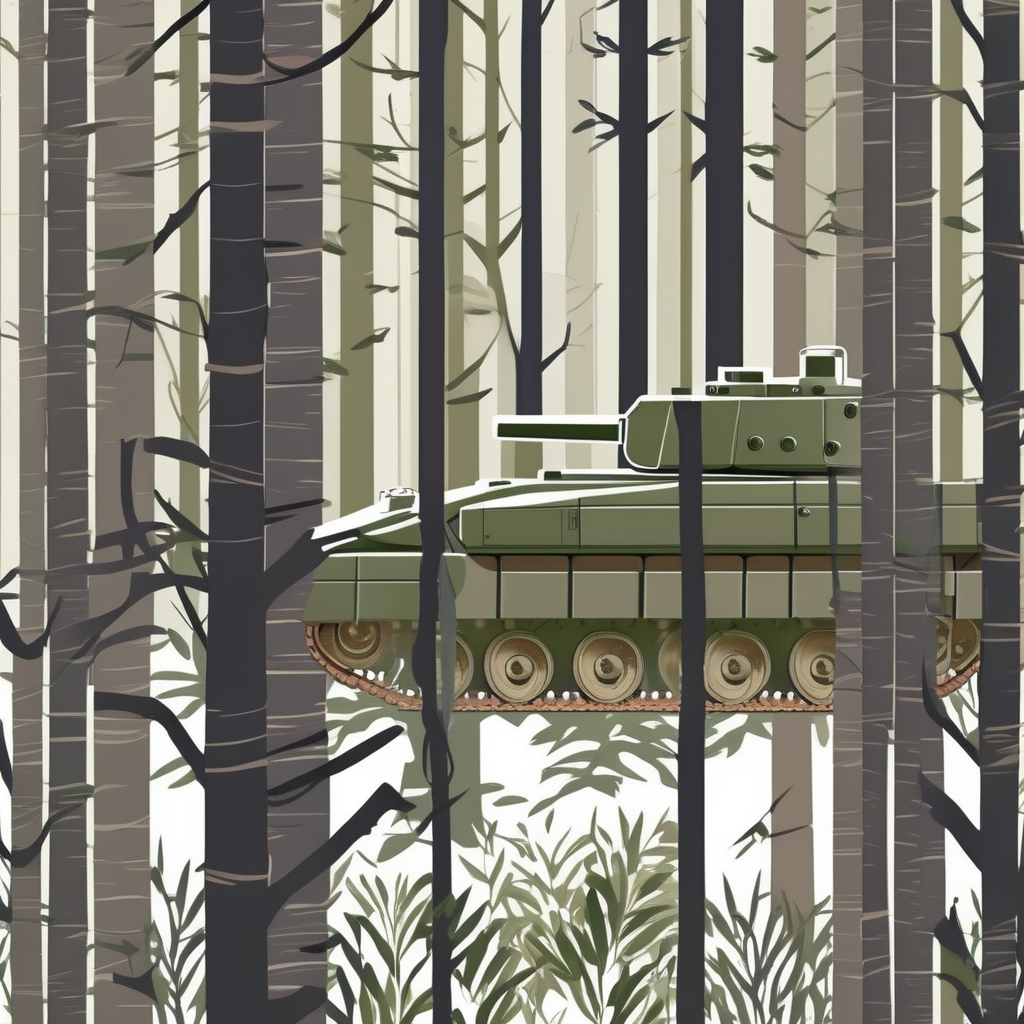
\includegraphics[height=5cm]{./images/tank-forest_camouflage-1.png}
    \end{subfigure}
    \hfill
    \begin{subfigure}[b]{0.45\textwidth}
        \centering
        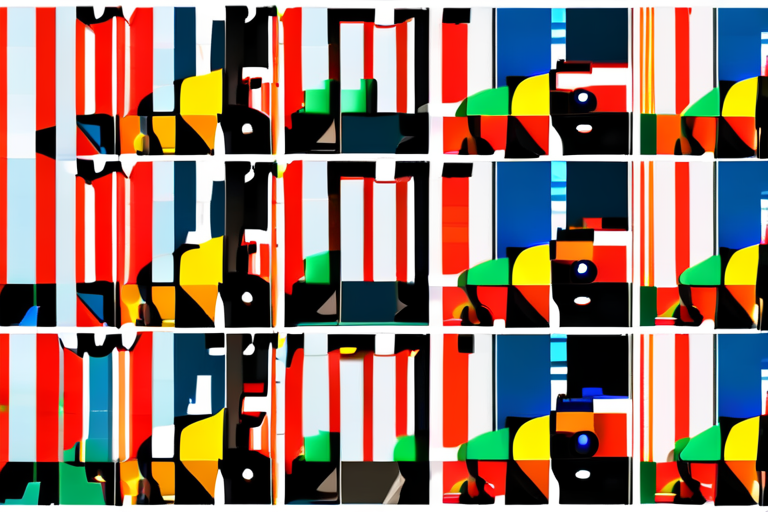
\includegraphics[height=5cm]{./images/tank-night_operation-1.png}
    \end{subfigure}
    \vskip\baselineskip
    \begin{subfigure}[b]{0.45\textwidth}
        \centering
        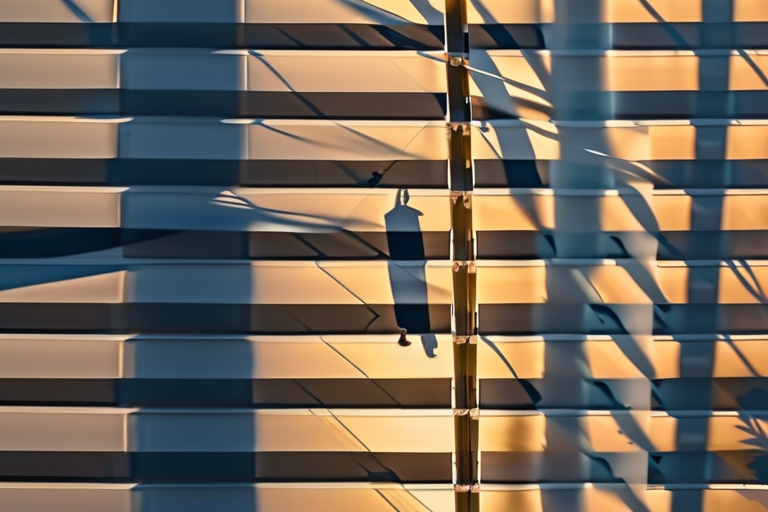
\includegraphics[height=5cm]{./images/tank-sunrise_maneuver-1.png}
    \end{subfigure}
    \hfill
    \begin{subfigure}[b]{0.45\textwidth}
        \centering
        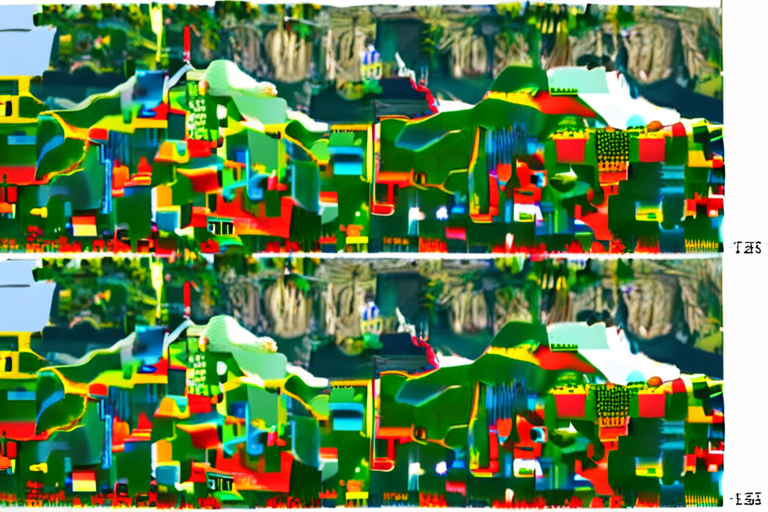
\includegraphics[height=5cm]{./images/tank-mountain_path-0.png}
    \end{subfigure}
    \caption{Exemples d'images synthétiques de véhicules militaires irréalistes et inexploitables}
\end{figure}

\section{Recommandations}
Nous avons proposer quelques pistes d'amélioration pour ce projet

\begin{itemize}
    \item \textbf{Transformation d'image:} Nous avons recommander dans un premiers temps de limité les transformations à 02 types par images au lieu de 03. Avec cela nous réduisons la probabilité d'obtenir des images complètement floues et inexploitable. En plus, cela peut nous permettre de faire de fois d'images en faisant des combinaisons de 02 types de transformations, nous aurons à la fin de la transformation 03 fois plus d'images dans le jeu de données.
    \item \textbf{Images synthétiques:} Stable diffusion V3 et XL, semblent générer des images moins réalistes de la version 1.5. On pourra se concentrer dans un premier temps sur cette version avant de passer aux versions plus récentes.
    \item \textbf{Jeux vidéos:} explorer la possibilité d'extraire des images de véhicules militaires dans des jeux vidéos.
    \item \textbf{Films d'actions/guerres: } En plus d'avoir des images réalistes, nous pourrons aussi avoir plusieurs images en situation complexe (camouflage, explosion, ...). Développer un outils permettant de couper des séquences vidéos contenant des scènes de guerres afin d'extraire le maximum d'images.
    \item \textbf{Vidéos des réseaux sociaux: } Scruter des publication pouvant contenir les images et ou vidéos contenant des véhicules militaires en situation complexe à reproduire.
\end{itemize}

Nous tenons à rester objectifs dans nos recommandations car, les images issues de ce travail, en majorité, ne seront pas annotées  et demandera donc un travail supplémentaire d’annotation manuelle, qui est souvent très coûteux (à minima en temps).
